\begin{figure}[htbp]
\centering
\captionsetup{
  justification=raggedright,
  labelsep=none,
  singlelinecheck=false,
  labelformat=boldlabel,
}
\caption[Figure 7: \footnotesize ]{\footnotesize \textbf{: Linear explainability of each ML model's predictions.} For each ML model (OLS, GLMNET, RF, XGB, NN1--NN3), the out-of-sample predictions are regressed on the signals (each cross-sectionally scaled to $[-1, 1]$ that month, hence approximately mean-zero) via the OLS global surrogate model. \emph{Left (intercept):} because the scaled signals are centred, the intercept is approximately the mean of the model's predictions -- its baseline predicted active return for a characteristic-neutral (median) stock. It captures the unconditional level of predicted active returns and also absorbs any level shift induced by the model's curvature (since it equals the average prediction, $\mathrm{E}[f(x)]$, not the prediction at the average, $f(\mathrm{E}[x])$); it is a common shift across stocks and does not affect the cross-sectional ranking. \emph{Centre (}$R^2$\emph{):} the share of prediction variance that is linear in the signals -- values near one indicate an essentially linear model. \emph{Right (residual variance):} the variance of the surrogate residuals, i.e. the part of the predictions the linear surrogate cannot reproduce. Together, $1 - R^2$ and the residual variance measure the nonlinearity and interaction structure the ML model captures beyond a linear function of the signals; both are near zero for the linear models (OLS, GLMNET) and larger for the tree and neural-network models. Values are for the final-refit surrogate on the individual-signals run.}
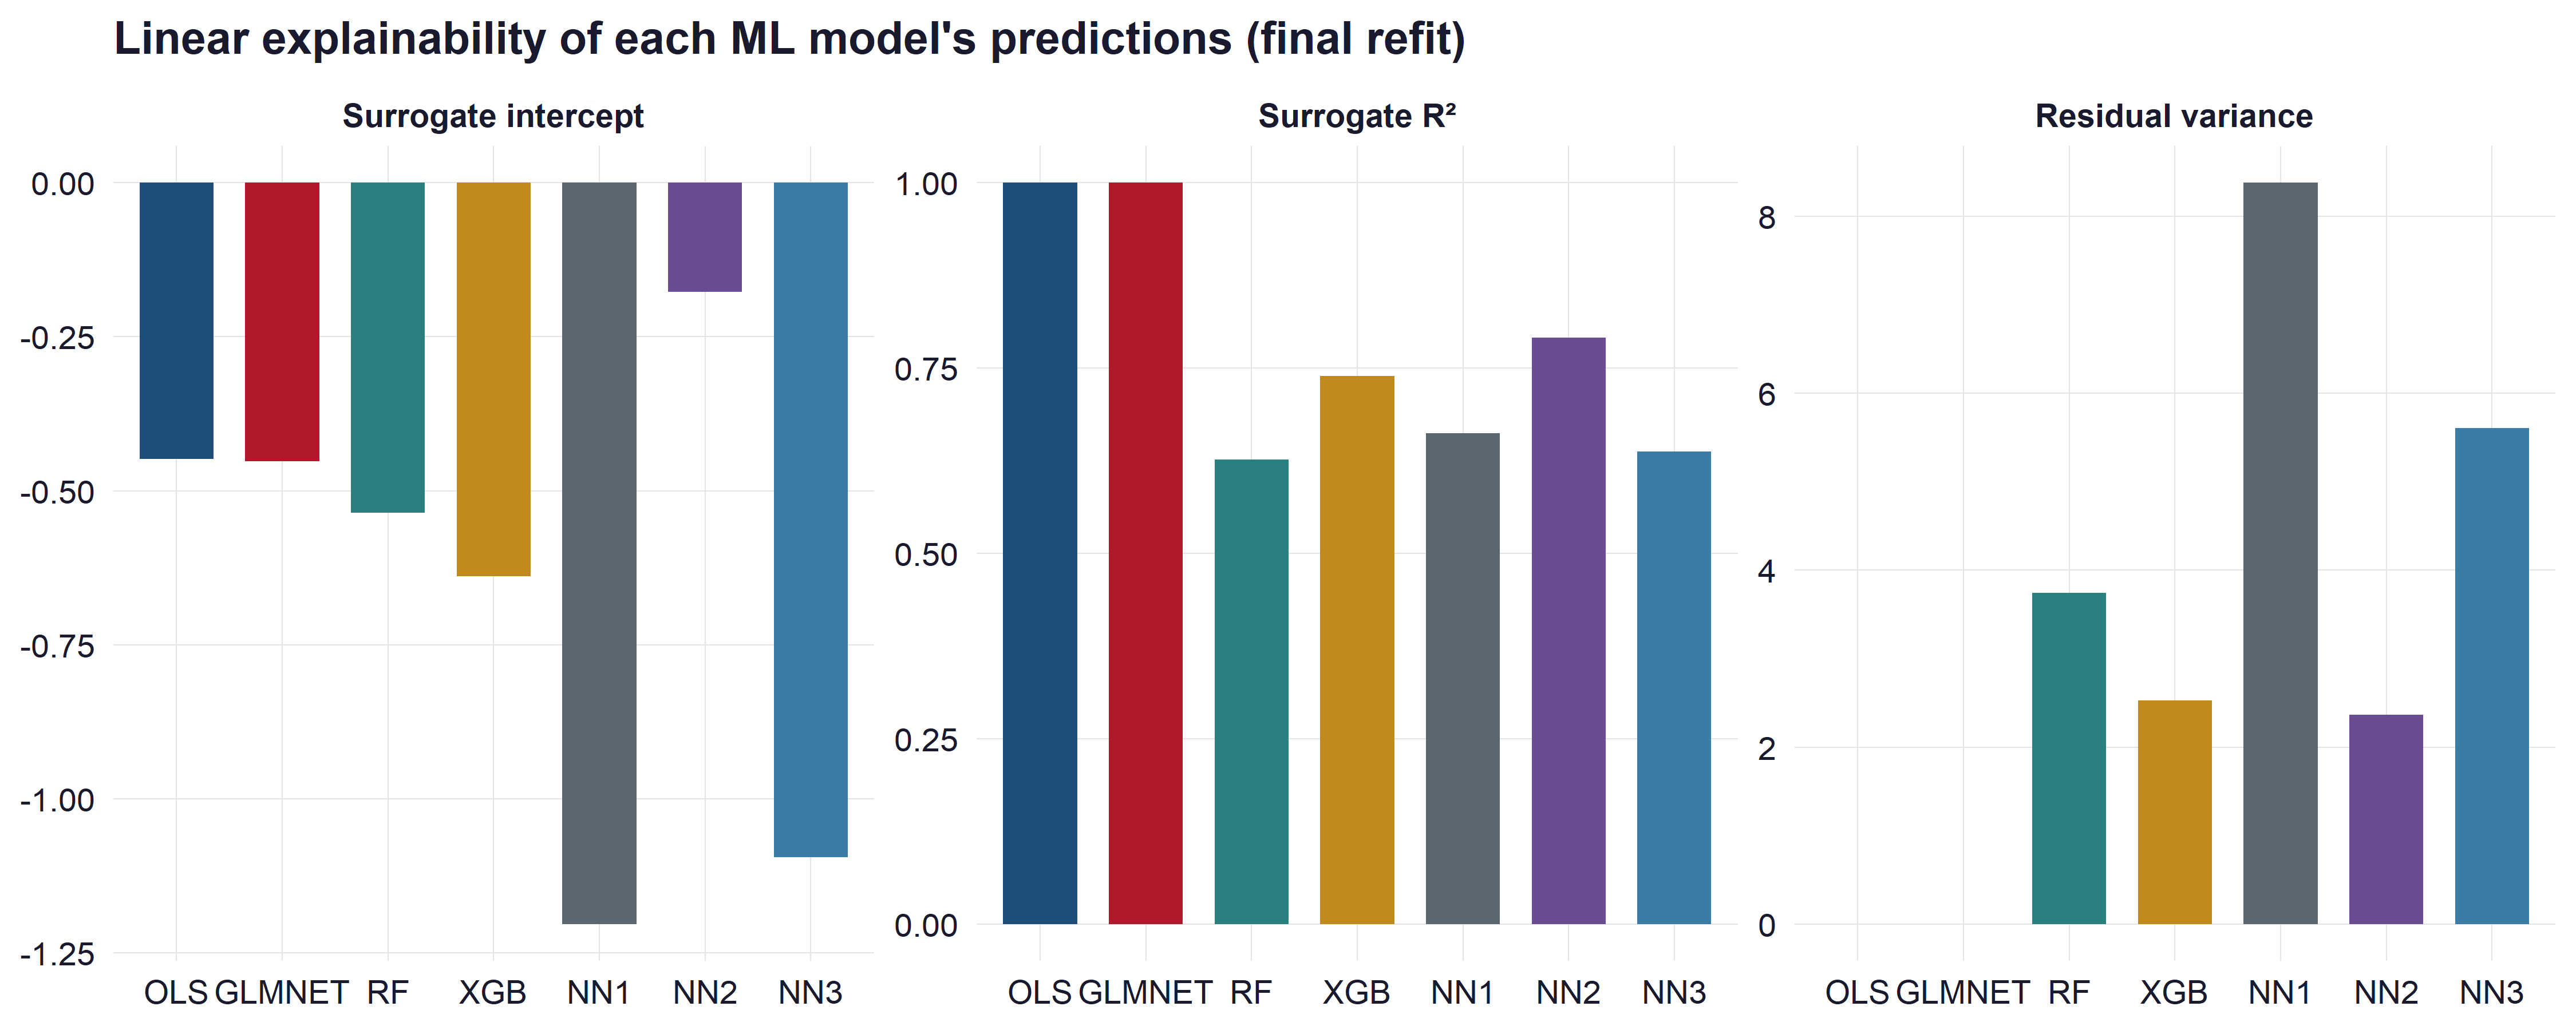
\includegraphics[width=\linewidth]{figures/surrogate_fit.png}
\label{fig:surrogate_fit}
\end{figure}
